\documentclass[heading.tex]{subfiles} 
\begin{document}

% \tableofcontents

\section{Introduction and Motivation}
Historically, there have been completely separate code-bases for design space exploration and
transient engine analysis. The capability to create flexible ``low fidelity'' models is ideal in
the earliest  conceptual design stages, where large design spaces can be explored relatively
quickly. As the engine design starts to become more concrete, higher fidelity models are
developed. These higher detail models are intrinsically more sensitive to design tweaks, and in
general take longer to setup. They inherently require more stringently defined sets of boundary
conditions and a specific configuration. A large variation in the baseline design could
potentially render entire higher fidelity analyses obsolete. Due to this weakness in adaptability,
higher fidelity models are generally not created until the low-fidelity design has fully matured.
This friction can partly be attributed to the differences in toolstes when transitioning to higher
fidelity models. 

\subsection{Design Cycle Overview}

	From a life-cycle perspective, there comes a point when the prospect of re-design becomes
prohibitively expensive and initial design decisions become cemented into the design. Any insights
gained from more detailed analyses are constrained to these initial design choices. Naturally, a
tradeoff exists on the amount of time spent in each analysis phase. Spending more time in the low
fidelity phase could have large payoffs in the long run; however, without higher fidelity models
it is hard to identify possible shortcomings such as those arising from operability and control
issues.

\begin{figure}[H]
\centering
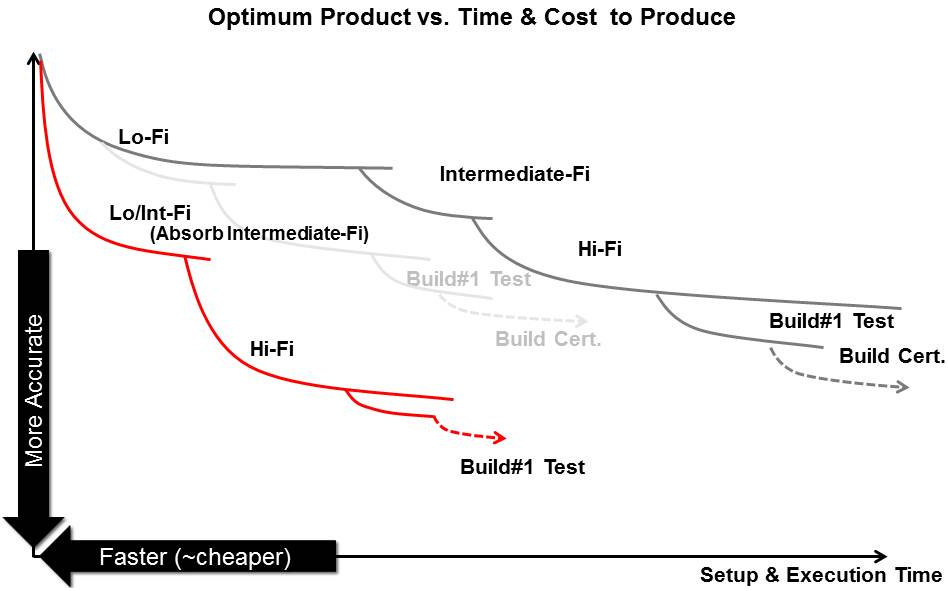
\includegraphics[width=1.0\textwidth]{images/optimum_product_vs_time}
\caption{Overarching Applied Research Challenge: Uncertainty in Optimum Product vs. Time \& Cost to Produce}
\label{f:product_vs_time}
\end{figure}

Figure \ref{f:product_vs_time} shows a pedagogical representation of the general relation between
accuracy and analysis set-up time. Lower fidelity (Lo-Fi) models are less accurate, but can be set
up and modified relatively quickly. The darker gray path characterizes the tradtional design
trend. Higher fidelity (Hi-Fi) models take longer to build, and therefore, aren't started until
the low fidelity model nears completion. If designers attempt to introduce Hi-Fi models earlier in
the design, as shown by the light gray line shifted to the left, they quickly become outdated as
the baseline model continues to undergo changes. Inevitably the models must be re-written to match
the new Lo-Fi design and the path reverts to the dark gray route. The only way to incorporate the
intermediate fidelity model earlier into the design process, is by absorbing the Int-Fi codes into
the low fidelity codes as portrayed by the red line. Combining both codes into a unified code
would accomplish this, but the codes can also be kept distinct as long as the Int-Fi model is
adaptable enough to keep up with the rapid changes of the Low-Fi code. Creating a single unified
code can also potentially become overly complex and cumbersome. A natural reaction is for various
disciplines to diverge and create unique tools satisfying their particular needs using frameworks
and programming languages that are already of familiarity. As mentioned earlier, this is
acceptable as long as the codes preserve flexibility and rapid adaptability. An intermediate
fidelity code can only be introduced earlier into the low fidelity analysis phase if it can keep
pace with the rapid redesigns.

The subsequent sections explore various design patterns to rapidly develop transient models. Each
approach starts with a base model built with NPSS, and assumes the reader already has a basic
understanding of how to construct a steady-state model. This paper focuses on further enhancements
required to interface NPSS with Matlab codes. The first method being the simplest and most
straightforward but performance constrained. The last being the most abstract. These methods
aren't mutually exclusive and the specific implementation details could vary greatly based on the
designer's discretion. 


\section{Running NPSS Transiently}


\begin{adjustwidth}{-1cm}{-1cm}
 \inputminted[]{c++}{code/transient1}
 \end{adjustwidth} 


Transient simulations represent the time-varying behavior of a system by finding a series of
solutions at discrete time steps over a desired time interval. NPSS solves these systems of
equations largely in the same way it handles steady-state solutions. However for transient
systems, some of the equations require integration rather than simply driving imbalances to zero. 

\subsection{Solver and Integration Methods}
NPSS supports multiple integration types, that are outlined in the NPSS users guide.
\cite[chap.~7.1]{NPSS} Table \ref{tab:Integration} summarizes the available methods, with a 
first-order differential equation for spool speed used as an example: 

\begin{minipage}{\linewidth}
\centering
\bigskip
\captionof{table}{NPSS Integration Methods} \label{tab:Integration}
\begin{tabular}{|c|c|c|}
\hline 
Method & Type & Solving for  $N_{t2}$, given  $N_{t2}- N_{t1}= \int_{t1}^{t2} \! \dfrac{T_{net}}{I} \, \mathrm{d}t $\\ 
\hline 
Euler & Explicit & $ \left.N_{t2}= N_{t1} + \dfrac{T_{net}}{I} \right|_{t1}^{}(t2-t1)$ \\ 
\hline 
Trapezoidal & Implicit & $ \left.N_{t2}= N_{t1} + \dfrac{1}{2}\middle(\dfrac{T_{net}}{I} \middle|_{t1}^{}+\dfrac{T_{net}}{I} \middle|_{t2}^{}\right)(t2-t1)$ \\ 
\hline 
$1^{st}$ Order Gear & Implicit & $ \left.N_{t2}= N_{t1} + \dfrac{ \mathrm{d}N }{ \mathrm{d}t } \right|_{t2}^{}(t2-t1)$ \\ 
\hline 
$2^{nd}$ Order Gear & Implicit & $ \left.N_{t2}= N_{t1} + \middle(\dfrac{1}{3}\dfrac{ \mathrm{d}N }{ \mathrm{d}t }\middle|_{t1}^{}+\dfrac{2}{3}\dfrac{ \mathrm{d}N }{ \mathrm{d}t }\middle|_{t2}^{}\right)(t2-t1)$ \\ 
\hline 
\end{tabular} 
\end{minipage}

Steady-state iteration may be required for any of these methods, and the choice between explicit
and implicit types comes down to accuracy vs time. Explicit methods assume the integrand is
constant over the specified time interval, therefore integration is only performed once per time
step. Implicit methods perform a sub-iteration (independent from time) until the predicted state
value agrees with the corrected value within a specified tolerance. NPSS also allows the user to
define custom integration methods using the \texttt{Integrator} class. \cite[chap.~15.2]{NPSS}  

\begin{adjustwidth}{-0.5cm}{-0.5cm}
 \begin{minted}{c++}
 setOption( "solutionMode", "TRANSIENT" );
 Transient.integrationType = "TRAPEZOIDAL"; //Default Gear 1st order
 transient.setup(); //run if changing to (or from) Euler method
 initializeHistory(); //run if initial conditions 
 	//differ from most recent transient run
 \end{minted}
 \end{adjustwidth} 
       

The top level transient solver is of type \texttt{TransientExecutive}, and is named
\texttt{transient} by default. This variable is analogous to the top-level steady-state 
``\texttt{solver}" object. The \texttt{transient} object is responsible for setting integration
solver properties including the simulation start, step and stop parameters. \cite[chap.~7.5]{NPSS}
\cite[chap.~15.1.8]{NPSS}  All attributes have a default value except \texttt{transient.stopTime},
which must be supplied by the user. Over the course of a run, the \texttt{TransientExecutive} may
update these attributes or even overwrite values set by the user. The user can also preemptively
stop a simulation using the  \texttt{quiescence()} and  \texttt{terminateCondition()} functions
available in the \texttt{TransientExecutive}.

\begin{adjustwidth}{0cm}{0cm}
 \begin{minted}{c++}
transient { //set as a group
	timeStepMethod = "ADAPTIVE";
	baseTimeStep= 0.10;
	dxTransLimit = 0.05;
	maxTimeStep = 0.20;
	minTimeStep = 0.01;
	stopTime= 3.60;
} //or set individually: transient.stopTime = 3.6;
 \end{minted}
 \end{adjustwidth} 

Before running transiently, the user must first ensure that each engine component with transient
specific attributes is properly initialized. Common components with special transient properties
include, shafts, springs, control volumes, heat exchangers, walls and thermal masses.
After steady-state engine sizing occurs, it is often necessary to determine multiple power
settings by running off-design cases, or trim the engine before initiating a transient. Once the
model is trimmed, the transient model is setup by adding/removing solver variables, setting
transient solver options, adding transient output viewers, and specifying time step and
termination criteria as described above.

\subsection{Transient Input}



\begin{figure}[H]
\centering
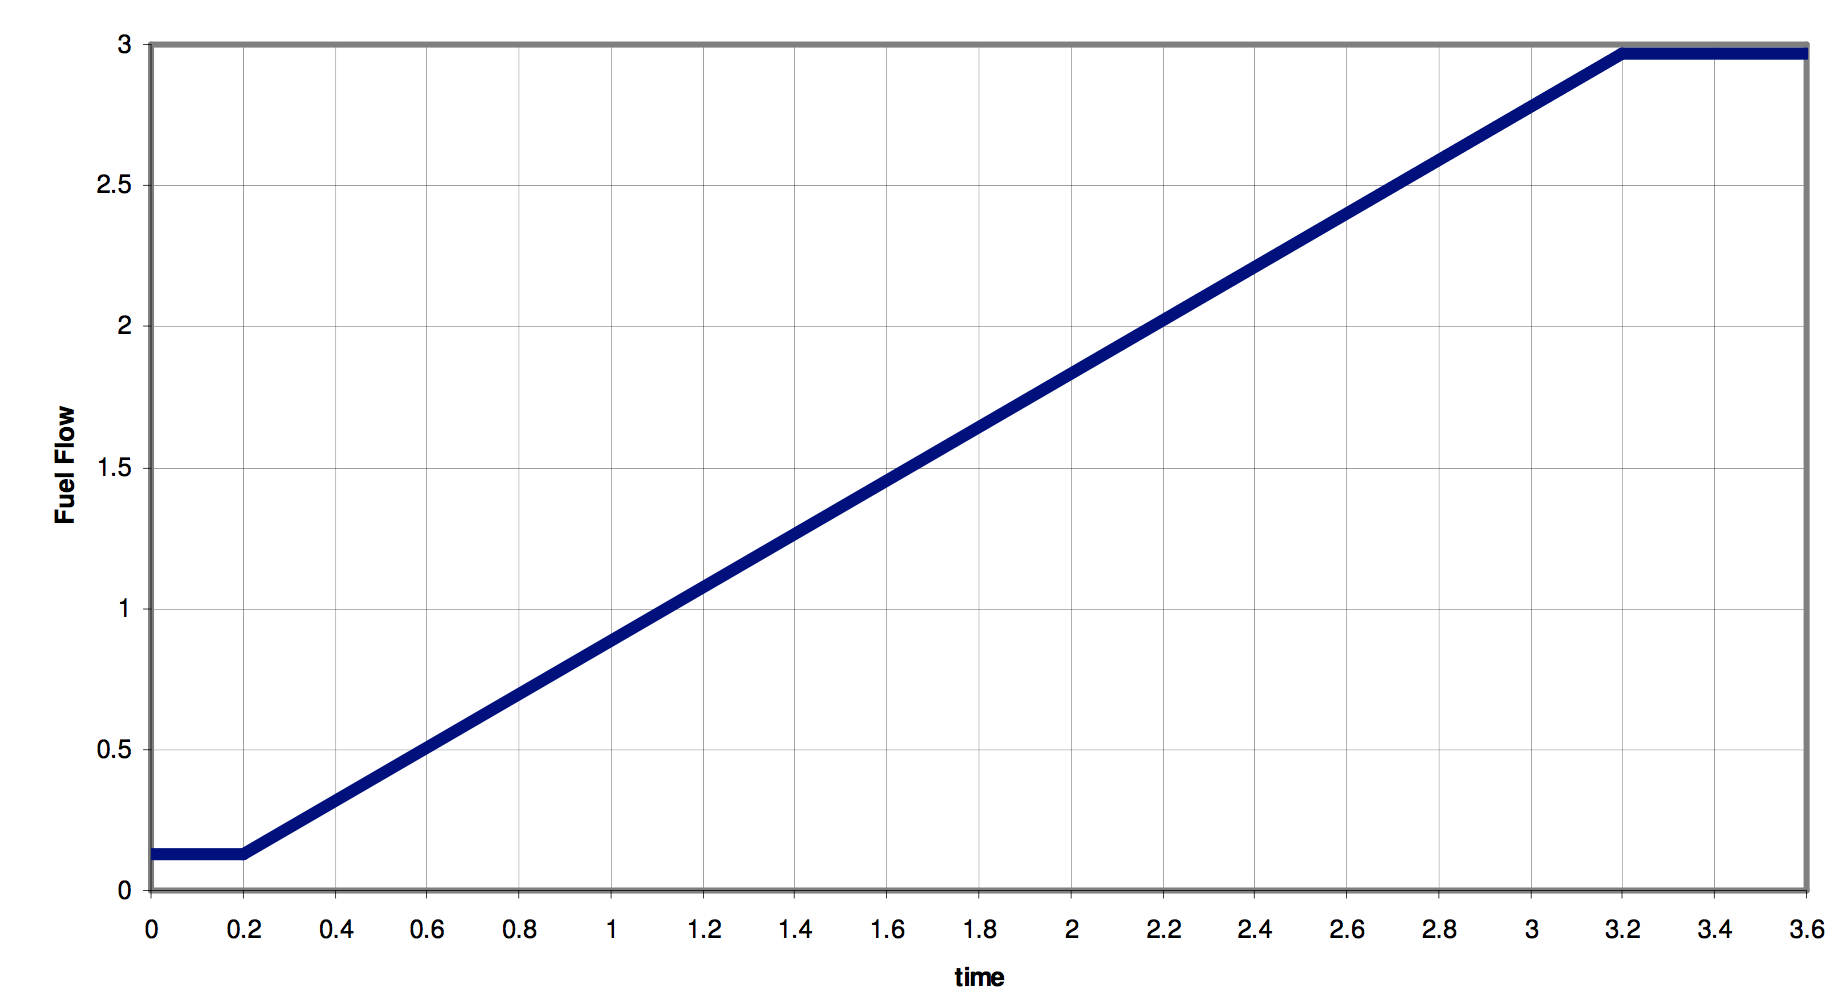
\includegraphics[width=1.0\textwidth]{images/fuelRamp}
\caption{Example fuel ramp used to drive a transient run}
\label{f:ramp}
\end{figure}

\begin{adjustwidth}{-1cm}{-1cm}
 \inputminted[]{c++}{code/rampFn}
 \end{adjustwidth} 
 
Or the same function could be built using a table. 
 
 \begin{adjustwidth}{-1cm}{-1cm}
 \inputminted[]{c++}{code/rampTb}
 \end{adjustwidth} 

Example code demonstrating all of these steps together can be found in appendix \cref{app:transient}.

\section{File Transfer}
\subsection{Batch Run}
This method involves:

\begin{enumerate}
  \item Specifying run cases in Matlab, programatically creating the batch and input files
  \item Transfer cases to NPSS
  \item Run Cases, output in matlab-syntax
  \item Transfer output back to Matlab
\end{enumerate}

\subsection{Transient}

Same process as above, except for every time step. Engine state saved to file.

\section{Compiled S-function}
\subsection{Background}
For Fixed Wing project, TTECTrA

Compatibility: R2008 - R2010b 32-bit only.

\subsection{NPSS Implementation}

The following solver variables are common in a steady-state and transient run of a turbofan
engine.

\begin{table}[H]
\centering
\begin{tabular}{|c|c|}
\hline 
Independent & Dependent \\ 
\hline \hline
\texttt{Ambient.ind\_W} & \texttt{Byp\_Nozz.dep\_Area} \\ 
\hline 
\texttt{Fan.S\_map.ind\_RlineMap} & \texttt{Core\_Nozz.dep\_Area} \\ 
\hline 
\texttt{HPC.S\_map.ind\_RlineMap} & \texttt{Fan.S\_map.dep\_errWc} \\ 
\hline 
\texttt{HPT.S\_map.ind\_parmMap} & \texttt{HPT.S\_map.dep\_errWp} \\ 
\hline 
\texttt{HP\_Shaft.ind\_Nmech} & \texttt{HP\_Shaft.integrate\_Nmech} \\ 
\hline 
\texttt{LPC.S\_map.ind\_RlineMap} & \texttt{LPC.S\_map.dep\_errWc} \\ 
\hline 
\texttt{LPT.S\_map.ind\_parmMap} & \texttt{LPT.S\_map.dep\_errWp} \\ 
\hline 
\texttt{LP\_Shaft.ind\_Nmech} & \texttt{LP\_Shaft.integrate\_Nmech} \\ 
\hline 
• & • \\ 
\hline 
• & • \\ 
\hline 
• & • \\ 
\hline 
\end{tabular} 
\caption{Solver Variables for a basic turbofan configuration}
\label{tab:SolverVariables}
\end{table}

Running with Dvariable flags.

Output: Solver.postexecute (transient user guide)

\subsection{Matlab Implementation}

\section{Source-to-Source Translation}
\subsection{Background}
Under the NASA Fundamental Aeronautics Program, the Supersonics Project is developing a variable
cycle engine (VCE) model for use in aero-propulso-servo-elastic (APSE) coupling studies of
supersonic vehicles. (Connolly, Kopasakis, \& Lemon, 2010) Analytical, computational, wind tunnel
and flight data of Aero-Servo-Elastic (ASE) systems have been thoroughly vetted however much work
still needs to be done to integrate propulsion dynamics into the ASE analysis tool suite.
(Fundamental Aeronautics Program Supersonics Project, 2006)
The Controls \& Dynamics branch and the Multidisciplinary Design, Analysis \& Optimization (MDAO)
branch at NASA Glenn are working in conjunction to produce a propulsion model that will eventually
be of a sufficient fidelity to directly couple with full-scale computational fluid dynamic (CFD)
and structural dynamic models. The task has been partitioned into three connected simulations: a
two-dimensional bifurcated inlet, a variable cycle turbofan engine, and variable area exit nozzle.
(Connolly, Kopasakis, Paxson, Stuber, \& Woolwine, 2012) 
Development of the engine simulation has proven difficult, largely due to the number of components
involved. Many of the challenges have been associated with data management issues or difficulties
in adaptability as the simulation has been scaled up in fidelity and engine complexity. The main
intent of this report is to discuss the strategies used to construct and initialize these large
models.  The methodology for computing component performance has been adopted from previous work
completed by the Controls \& Dynamics group, (Kopasakis, Connolly, Paxson, \& Ma, 2008) and is
beyond the scope of this paper.
This report focuses on a novel software generation tool being designed to dramatically reduce
engine model set-up time, allowing higher fidelity analyses to be introduced earlier in the design
cycle. The software is intended to work for any type of engine architecture, but was originally
tailored for the VCE configuration. The benefits of the tool are most apparent when its impacts
are framed from a design cycle standpoint.

	In the context of NASA Glenn’s supersonic program, the Numerical Propulsion System Simulation
(NPSS) VCE engine is the low fidelity model, and the Supersonic Component Engine Model (SCEM) is
the intermediate fidelity model. The NPSS model is a framework written in C++, while the SCEM
model is developed within the Matlab/Simulink environment. The SCEM model performs its own unique
calculations, but requires the steady-state engine characteristics of the NPSS model to initialize
the simulation. Large advances needed to be made to the intialization scripts of the SCEM program
if both programs are to be run congruently. A brief history of the SCEM model is provided below to
shed light on the amount of work that is required to build such a model and to emphasize the clear
need for improved extensibility.  

\subsubsection{Problem Decomposition}

Although the SCEM solver is fundamentally different, both models are comprised of the same
thermodynamic elements, linked together in the same order. Historically, the SCEM model has been
built up manually, element-by-element within Simulink based on the NPSS model architecture. After
building the engine “skeleton” within Simulink, flow station properties and performance maps
generated by NPSS were manually scaled, transferred, and then saved into the Matlab workspace.
These variables were stored in large multi-dimensional matrices which then needed to be resaved
with unique “human-understandable” names so that they could be manually connected to the Simulink
engine. This process was extremely time-intensive and error prone. Furthermore, everything was
programmed procedurally with a very specific sequence. This meant that any additions or
modifications to the engine design would require every variable to be modified or re-arranged
based on the new design. In order to automate the generation of an analogous SCEM model, the
program needed to adopt the same object-oriented nature of NPSS. After aligning the framework
paradigms between NPSS and SCEM, it was possible to create a parallel Matlab “objects” for each
pre-made element contained within NPSS. These Matlab objects contain all of the data book-keeping,
calculations and Simulink structures necessary to build many of the common elements within NPSS.
This automates the conversion of any NPSS model into an analogous Matlab model, greatly reducing
the opportunity for human error, and makes the framework much easier to modify. The implementation
details for these Matlab objects are described in detail in subsequent sections of this report.	


\subsubsection{Program Goals and Future Development}

The automated Matlab/Simulink code generator was originally designed to aid in the construction of
the VCE engine for the APSE project; nonetheless it can theoretically be applied to any NPSS
model. As long as NPSS provides a consistent method for passing information, a Matlab object can
be created for every NPSS element and beyond. In order for the code generation tool to be useful
it will need to be as flexible as NPSS. The object-oriented nature will hopefully make this easy
by providing well-defined interfaces between the various component objects for developers, while
hiding the unnecessary implementation details from the user. The modularity of each element will
allow the program to be updated incrementally, and conversely, large program-wide changes can be
implemented simultaneously for all elements of the same type. 
	A second revision of the program will hopefully allow it to dynamically communicate with NPSS
providing balanced engine calculations on demand. A closer integration would eliminate the need
for large interpolation tables, allow for better suited data transfer and possibly increase the
speed and accuracy of the program.

\subsection{NPSS Implementation}

NPSS engine models vary widely in file organization and implementation details depending on the
model builder. The core commonality between models is the standard set of engine components and
the fluid and socket connections made between them. The custom functions created for this tool are
designed to be non-intrusive, and compatible with the wide variety of programming styles used to
build an NPSS model. The functions can easily be appended to existing models and only require a
small amount of user input to provide MATLAB with information that can’t be gleaned automatically.
All NPSS output is user-defined, so these custom functions were created to output engine data in a
format easily manipulated by Matlab and indexed in a manner that is still human-readable. The
three custom functions and their output are described below.

\subsubsection{NPSS to Matlab Run File}

After constructing the notional engine architecture in NPSS, run files are used to carry out
calculations and direct workflow in engine resizing, analysis and optimization. A MATLAB specific
run file was created to be appended to existing run files, allowing the engine to be run through
all the operating conditions of interest and output files to be used by MATLAB. The script sets
the appropriate independents/dependents to solve the simulation and then runs a single design
point to size the engine. Next, a series of off-design conditions are run to create a large matrix
of possible operating conditions across the flight envelope. A WATE++ model is then run to
generate the corresponding physical engine design. All of the pertinent information is then output
to MATLAB files. The MATLAB run file also includes an optional file that can be generated by
MATLAB before NPSS runs. This allows a user in the MATLAB environment to specify flight envelope
run cases of interest, then run NPSS all from within the MATLAB workspace. More information on the
workflow to pass from MATLAB to NPSS back to MATLAB can be found in the “Run NPSS” section of the
Matlab implementation section.

\subsection{Matlab Implementation}

\subsubsection{Component Library}

Similar to NPSS, a library of generic engine elements was composed to handle many combinations and
engine architectures. These custom Matlab classes use object-oriented features that first became
available in the R2008a revision of Matlab (The MathWorks Inc, R2013a), a language that primarily
supports a more procedural programming paradigm. An object is a specific instance of a class,
which follows the basic blueprint of the class, but with its own internal properties. Each
component class is complimented by a generic Simulink subsystem model. When an object is
instantiated and loaded, the component subsystem is added to the overall Simulink model. Each
class “book-keeps” data pertinent to that component type, and controls the behavior of the loaded
Simulink model. These classes help to keep the otherwise unwieldy amount of incoming data
organized, and allow the engine to be constructed automatically based on an equivalent NPSS
engine. Using a relatively small number of instructions (automatically generated by the NPSS
output described above) an entire Simulink engine can be constructed from various component
instances, be fully connected to each other, with every subsystem appropriately populated.

	The inherent modularity of the component library allows new classes to be added or modified
without affecting the rest of the library, while simultaneously allowing modifications to be made
across every instance of a particular class without duplicated effort. A system-wide bug affecting
every duct element in an engine could be addressed in a single piece of code, while still offering
the ability to tailor individual instances of ducts with various configurations and attributes.

\section{Final Remarks}
This is conclusions section it's quite handy.


\end{document}

%%% Local Variables: 
%%% mode: latex
%%% TeX-master: t
%%% End: 
